
\begin{IEEEbiography}[{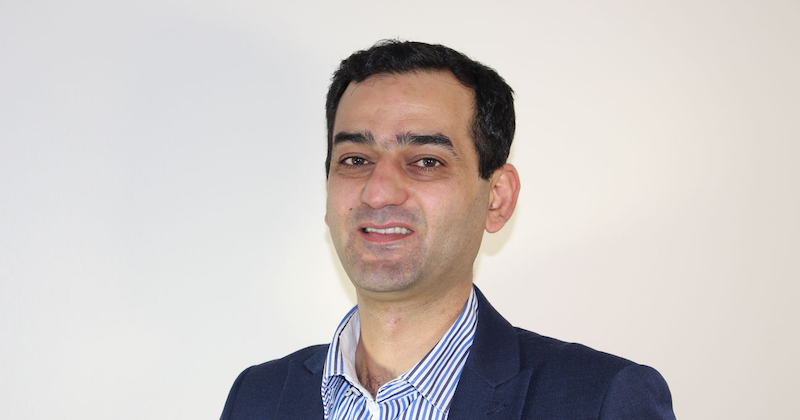
\includegraphics[width=1in,height=1.25in,clip,keepaspectratio]{a1.png}}]{Basel Magableh} 
Dr. Basel Magableh is  Lecturer in the School of Computer Science, Technological University Dublin. Basel has a BSc from the University of Yarmouk, Jordan, MSc from New York Institute of technology, USA and a PhD from Trinity College Dublin, Ireland. Basel has previously worked as a Chief Scientist in Mobile/Terminal Context Awareness in Huawei Technologies, Finland. He has also completed two post doctorate positions in UCD, and the Knowledge and Data Engineering Group (KDEG), Trinity College.
\end{IEEEbiography}

\begin{IEEEbiography}[{
\includegraphics[width=1in,height=1.25in,clip,keepaspectratio]{a3.png}}]{Muder Almani} 
Dr. Muder Almani is a Chair, Computer Information Systems Department / College of Information Technology Chair, Management Information Systems Department / College of Business Administration and Economics, Al-Hussein Bin Talal University, Ma'an - Jordan. Muder is actively researching in document handling, modems, peer-to-peer computing, power amplifiers, redundancy, security of data, storage management
\end{IEEEbiography}

\begin{IEEEbiography}[{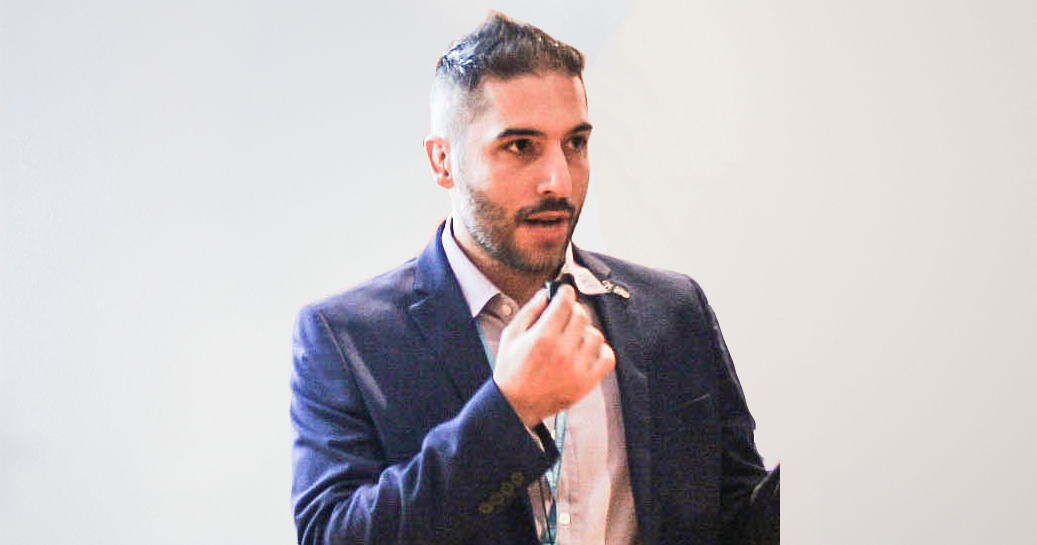
\includegraphics[width=1in,height=1.25in,clip,keepaspectratio]{DrLucaLongo380x200.png}}]{Luca Longo}  
Dr. Luca Longo is Lecturer in the School of Computer Science, Technological University Dublin.
Luca interests have always turned around Artificial Intelligence and innovative applications, especially applied to formal reasoning and the World Wide Web. Luca have completed a BSc with honours and a MSc awarded distinction both in Computer Science at the University of Insubria (Varese, Italy). Luca have obtained also a Postgraduate Diploma in statistics and a MSc in Health Informatics awarded distinction at Trinity College Dublin (Ireland). Luca successfully defended  PhD thesis in Artificial Intelligence at Trinity college Dublin. Additionally, Luca have recently obtained a Postgraduate diploma in Learning and Teaching at Dublin Institute of Technology, where Luca currently am tenured lecturer, covering both MSc and PhD courses.

Luca vision  is to formalise the ill-defined construct of human Mental Workload as a computational concept through deductive knowledge representation and reasoning techniques (Defeasible reasoning, Argumentation Theory) and inductive modelling techniques (Machine Learning). Field of applications includes Human-Computer Interaction, Education, NeuroScience, Universal Design.
\end{IEEEbiography}


